\section{Assessing Risk Preferences: A Dual-Criterion Approach}
\subsection{Setup and Definitions}
The results of section \ref{return_section} paint very different pictures of retail investors. 
Using the method set forth by \cite{Welch2022} and \cite{Fedyk2024}, analyzed also in section \ref{fedyk_paper_returns}, yields superior returns and similar drawdowns to the market.
They also conclude that the Robinhood crowd has achieved positive alpha when analyzed under different factor models (table VII, IX, X in \cite{Welch2022} and table 16 in \cite{Fedyk2024}). 
These results appear to be in contrast with the existing literature on retail investing, most notably \cite{BarberOdean2000}.

A more fundamental question, however, is whether those returns are attractive once investors' attitudes toward risk are taken into account.
This section evaluates the Robinhood portfolio against its market benchmarks using two complementary criteria.

First, I adopt the constant-relative-risk-aversion (CRRA) framework, in line with the majority of asset pricing work.
\begin{equation}
    U(W) = 
    \begin{cases}
    \frac{W^{1-\gamma}-1}{1-\gamma}, \gamma\neq 1\\
    \ln(W), \gamma = 1
    \end{cases}
    \label{CRRA}
\end{equation}

By computing the expected utility of both the Robinhood and benchmark portfolios over a grid of possible risk aversion ($\gamma$) values,
I identify the cutoff $\gamma^*$ such that a representative CRRA investor is indifferent between the two.
This delivers a concise, parametric summary of how risk preferences may shape portfolio choice.

Then, I estimate the welfare loss derived from investing in the Robinhood portfolio rather than (i)  not investing or (ii) investing in the market portfolio.
By comparing the certainty-equivalent wealth under each strategy for a CRRA investor, with risk aversion calibrated inside a feasible range,
I obtain dollar-denominated welfare losses that capture the risk-return profile taken by Robinhood investors.

To account for the uncertainty deriving from the limited sample size and high variance we employ also another approach to estimate risk-aversion. 
We directly estimate the risk aversion $\gamma$ from the percentage of wealth invested in the risky asset ($\alpha$), 
precise numbers about the wealth of Robinhood investors are not available, we therefore plot the implied risk aversion over a grid $\alpha$ and compare it to alternative portfolios.
It must be explicitly stated that in all sections, except this last, it is assumed that investors are entirely invested in the risky asset.

\subsection{Expected Utility and Cutoff}
\label{sec:cutoff}
%\subsubsection{Sampling Variability and Finite-Sample Limitations}
Identifying a cutoff level of risk aversion provides a clear criterion for the CRRA utility-maximizing investor: 
it is the minimum $\gamma$ at which an alternative strategy becomes preferred to the Robinhood portfolio.
However, the limited size and noise of the sample imply wide conference intervals for the estimated expected utilities at different $\gamma$ levels.
In practice, this remains a useful conceptual framework to understand how risk preference and beliefs may affect portfolio choice, but in limited samples, its numerical outputs are more illustrative than definitive.

Formally, we want to find $\gamma^*$ defined as:
\begin{equation}
    \gamma^* = \min\left\{ \gamma_j : \mathbb{E}[U_p(\gamma_j)] \leq \mathbb{E}[U_m(\gamma_j)] \right\}
    \label{gamma_cutoff}
\end{equation}
where $U_p(\cdot)$ is the utility of the Robinhood portfolio, while $U_m(\cdot)$ is the utility of the market portfolio.

In practice, we apply CRRA utility function (\ref{CRRA}) to each gross return observation and then takes the sample average.
The resulting mean serves as the expected utility implied by the investor's revealed choices over the sample period.
Wealth at time $t$ is equal to gross returns, assuming the initial wealth $W$ to be equal to one without loss of generality.


The main problem related to this approach is inherent to the sample we apply it to, having only 539 observations and inclusion of extreme events such as the COVID crash. 
These factors inflate the sample variability of our mean-utility estimates. 
Therefore, the resulting confidence intervals for the sample mean remain wide. 

We don't pretend to draw absolute conclusions but a few noteworthy remarks must be stated.
We compare the two Robinhood portfolios with the S\&P 500 and the Wolrd ETF, resmapling returns every $n$ days instead of taking rolling returns to avoid distortions due to autocorrelation. 
First, the Fedyk approach yields higher $\gamma^*$ values than my approach across comparable horizons and market proxies.
This can be interpreted as a relative perfomance index, telling us that if we accept the approach based directly on prices, then Robinhood investors would need to have lower risk aversion 
to not be convinced to hold the market.

Remarkably, investors with a risk aversion paramter even slightly lower than 1 would have a higher utility by investing in the S\&P 500 rather than in the "Mine" portfolio.
Fedyk's portfolio requires a risk aversion between 1.7 and 2; more plausible values although relatively low to empirical estimates.
When comparing the two Robinhood portfolios with the World ETF, the values for $\gamma$ increase in the 2-4.2 range, 
higlighting a less attractive performance of this ETF when compared to the Robinhood portfolios.
Detailed estimates can be found in table \ref{tab:cutoff_gamma}.

The key takeaway from comparing the two Robinhood-based portfolios is that Fedyk's construction systematically requires a 
higher level of risk aversion before the market overtakes it than the "Mine" strategy does. 
In practical terms, this means that Fedyk's portfolio must be judged by a much more cautious investor before traditional market benchmarks become more attractive. 
Under Fedyk's construction, only investors with high risk aversion would prefer the S\&P 500 (or the World ETF) to the Robinhood-style basket; those with moderate risk aversion could rationally stick with the Robinhood mix.

By contrast, the "Mine" portfolio flips that relationship. 
Its cutoff $\gamma$ is much lower, which implies that even investors who are only mildly risk-averse would already find the market to deliver higher expected utility than our version of the Robinhood strategy. 
In other words, this portfolio construction leaves fewer "justifiable" investors: only the very least risk-averse would stick with it once they properly account for risk preferences.



%\subsubsection{Augmented Return Sample via All Date-Pairs}
%\label{sec:allpairs}
%To overcome the limited information in only 539 daily observations, we construct an "all-pairs" dataset that dramatically amplifies our effective sample.  
%Specifically, let the trading-day indices in our original series be $1,2,\dots,T$.  
%For every ordered pair of dates $(i,j)$ with $1 \le i < j \le T$, we compute the cumulative excess return (net of the risk-free rate) between day $i$ and day $j$ as
%\begin{equation}
%    R_{i,j}
%    \;=\;
%    \prod_{k=i+1}^{j}\bigl(1 + r_k - r_{f,k}\bigr),
%    \quad
%    1 \le i < j \le T,
%    \label{eq:allpairs_return}
%\end{equation}
%where $r_k$ is the portfolio return on day $k$ and $r_{f,k}$ is the daily risk-free rate.  
%Using excess returns over the risk-free rate is necessary due to the changes in macroeconomic policy during the time of the sample. 
%We treat each multi-day return $R_{i,j}$ as a separate outcome in the investor's distribution of possible holding-period returns, we increase the number of observations from $T$ to $T(T-1)/2$, which reduces sampling variability in our utility-based estimates.  
%This "all-pairs" approach preserves the time-ordering of returns while allowing us to evaluate expected utility cutoffs with far greater precision.  
%
%In practice, this results in finding a very low $\gamma^*$ that satisfies equation \ref{gamma_cutoff}, meaning that every investor with a reasonable risk-aversion parameter under CRRA utility would have a greater utility by investing in the market\footnote{
%Both the risk-free rate and market returns are downloaded from Kenneth R. French data library \url{https://mba.tuck.dartmouth.edu/pages/faculty/ken.french/data_library.html}}.
%In some cases, particularly when ending the sample before the pandemic, the utility curves fitted on the "all-pairs" dataset simply do not intersect for a wide grid of possible risk aversion,
%and in fact we find also that in these cases the market stochastically dominates the robinhood portfolio (something which will be analyzed more in depth later).
%
%Performing this exercise for the whole period on the two alternative Robinhood portfolios yields very telling results.
%In both instances the cutoff risk aversion as defined in \ref{gamma_cutoff} is negative; 
%in particular, the portfolio I constructed has a cutoff risk aversion of -5.437 while the one built using the alternative method we obtain -5.239.
%The plot below shows this finding, only extremely risk loving investors would prefer the Robinhood portfolios over a diversified index.  
%
%\begin{figure}[H]
%  \centering
%  \subfloat[Robinhood Returns Built from Prices]{%
%    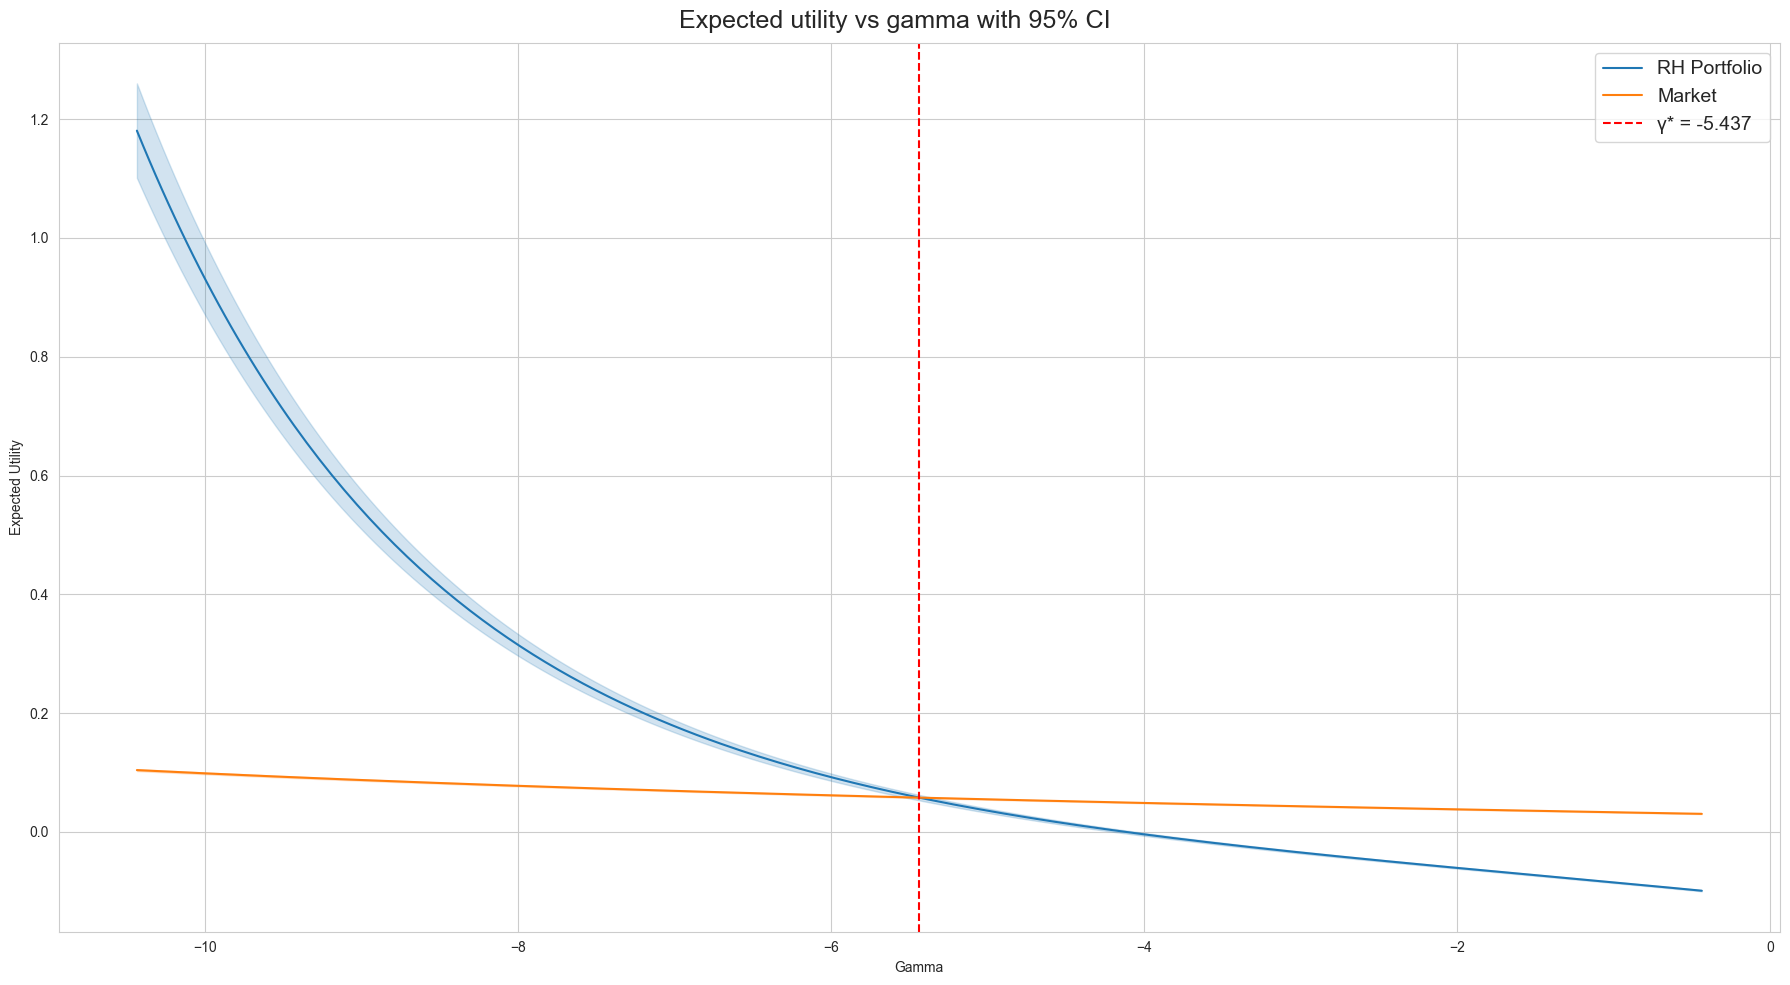
\includegraphics[width=0.48\textwidth]{../images/risk/cutoff_number_all.png}%
%    \label{fig:cutoff_number_all}
%  }
%  \hfill
%  \subfloat[Robinhood Returns Built Following Fedyk]{%
%    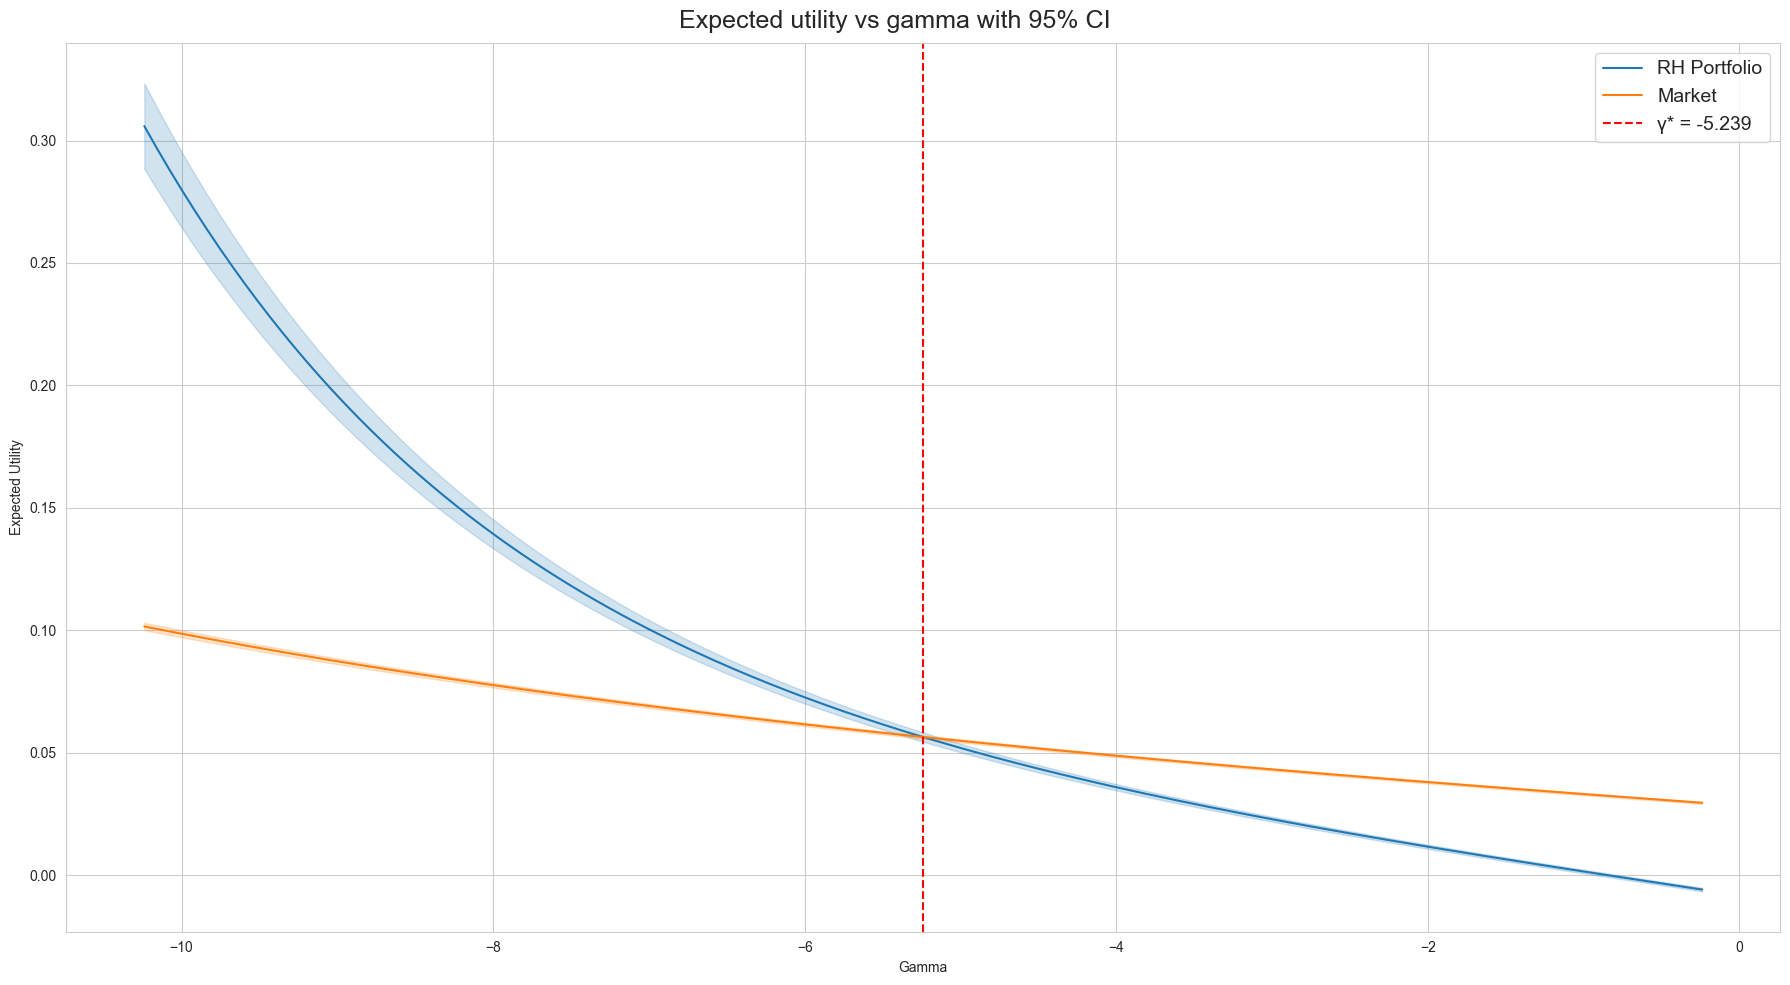
\includegraphics[width=0.48\textwidth]{../images/risk/cutoff_wealth_all.png}%
%    \label{fig:cutoff_wealth_all}
%  }
%  \caption{Expected Utility and Cutoff Risk-aversion for the Robinhood and Market Portfolio.}
%  \label{fig:cutoff_all_sidebyside}
%\end{figure}
%
%The only case in which $\gamma^*$ is positive is when we compare the Fedyk Portfolio and the World equity ETF as a proxy for the market index, obtaining a value of 1.214.
%This implies that weakly risk-averse and risk-loving investors would have a greater utility by investing in this index.
%However, if we limit the analysis to the pre-COVID period, the utility of the World ETF strictly dominates for each $\gamma\geq-15.813$, 
%highlighting that the former result might indeed be a result of the volatility experienced in early 2020.  

\subsection{Computing Welfare Loss}
In this section, we want to estimate the Welfare loss from investing in the Robinhood portfolio rather than in the market or in the risk-free asset.
The goal is to give a quantitative measure of the behavioral cost of choosing one strategy over another.
In other words, how much would we have to pay a Robinhood investor to make them switch to another portfolio?
We perform this analysis comparing the Portfolio formula set forth in this paper and Fedyk's against the world ETF, the S\&P 500, and the risk free asset. 

To compute the welfare loss we first need to derive the certainty equivalent for the CRRA function.
Starting from the definition of certainty equivalent and \ref{CRRA}:
\begin{align}
\begin{split}
    U(CE) &= \mathbb{E}[U(W)] \\
    CE &= \left[\mathbb{E}(W^{1-\gamma})\right]^{\frac{1}{1-\gamma}}
\end{split}
\label{ce_crra}
\end{align}

Then we define the welfare loss for a certain risk aversion parameter $\gamma$ as:
\begin{equation}
    WL_{\gamma} = CE_{p, \gamma} - CE_{b, \gamma}
\end{equation}

Where $CE_{p, \gamma}$ and $CE_{b, \gamma}$ are respectively the certainty equivalent of the portfolio and the base strategy to which we compare it, both evaluated for a certain $\gamma$.
In practice, $WL_\gamma$ quantifies the least riskless returns we would need to pay to an investor with a certain $\gamma$ to make them switch to the alternative strategy.

\paragraph{Welfare Loss Compared to the Risk-Free Asset}
When we benchmark each strategy against the the risk-free asset, every risky portfolio must bear a positive welfare loss for sufficiently high risk aversion. 
The S\&P 500 suffers the smallest penalty, the green curve stays closest to the zero line, implying that even moderately risk-averse investors would demand only a small payment to forsake cash for the index. 
The World ETF lies slightly below, so it too outperforms the Robinhood baskets but at a marginally higher cost in utility relative to the risk-free benchmark.

Both the "Mine" and Fedyk portfolios incur substantially larger losses.
At very short horizons, all strategies look similar, the noise of one-day returns dominates, but as we move to 30- and 60-day periods the cost of volatility in the Robinhood portfolios grows sharply. 
Mine has the steepest utility price, particularly for investors with $\gamma$ above one or two. 
Fedyk lies between the market indices and my version of the Robinhood mix.

In practical terms, an investor with moderate aversion to risk ($\gamma$ around two) would be willing to pay only a few basis points of expected return to switch from VT or the S\&P 500 into cash, while they would demand markedly larger compensation to move from the Robinhood portfolios back into risk-free assets. 
This ordering confirms that, although both Robinhood strategies can outperform in raw returns, their behavioral cost relative to cash is significantly higher than that of mainstream market ETFs.
Notably, we can highlight the fact that the behavioral cost for investing in Fedyk's portfolio is lower for a wide range of $\gamma$.
\begin{figure}[H]
    \centering
    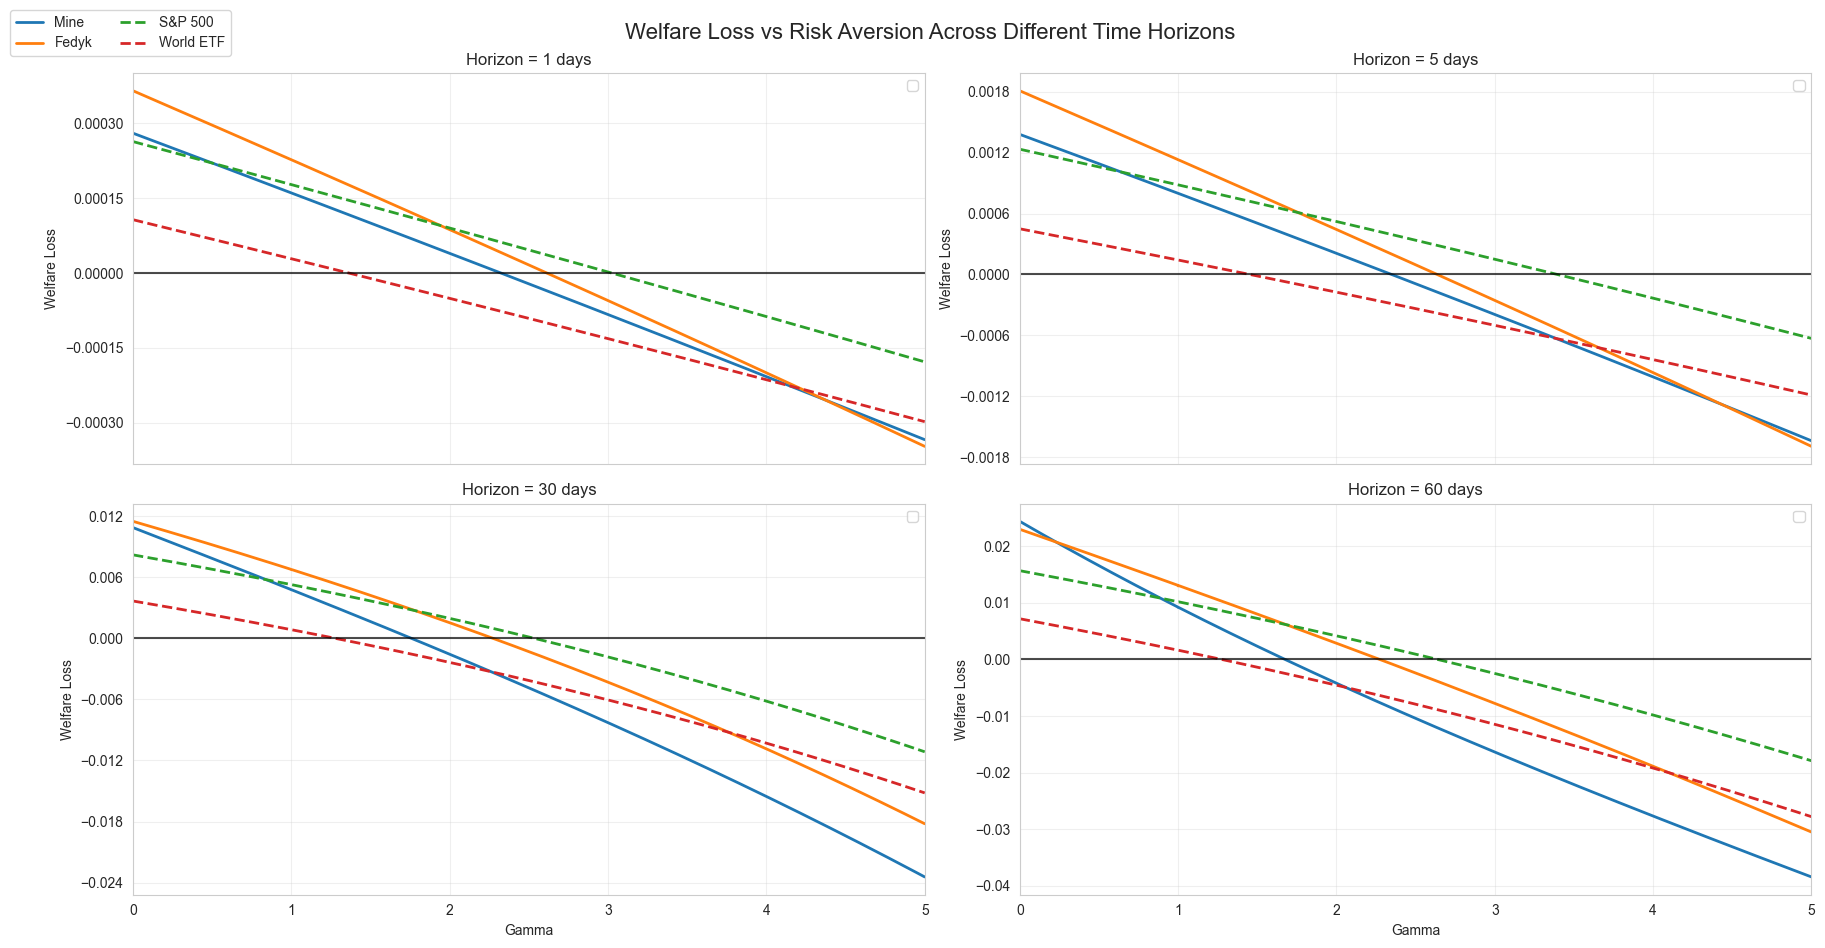
\includegraphics[width=\linewidth]{../images/wl_rf.png}
\caption{Welfare loss relative to a risk-free asset for four strategies plotted as a function of the CRRA risk-aversion coefficient across 1-, 5-, 30-, and 60-day return horizons.}
\end{figure}    



\paragraph{Welfare Loss Compared to Market Indeces}
When we measure each Robinhood proxy against the two broad market benchmarks, striking differences emerge in how quickly risk-aversion erodes their advantage.  
At $\gamma=0$ (risk neutrality), all four curves start above zero—indicating that a completely risk-neutral investor would prefer any of the Robinhood strategies to either the World ETF or the S\&P 500.  
Figure \ref{fig:wl_mkt} confirms what we've jsut described.
First, "Mine" has a higher behavioral cost compared to Fedyk's construction.
Secondly, taking the World ETF as a proxy for the market instead od the S\&P 500 implies even greater behavioral costs.
Lastly, as the horizon increases the value of $\gamma$ for which the welfare loss is zero decreases, implying that the certainty equivalent of the Robinhood Portfolio, however computed, falls short of that of the market very quickly and for a wider array of investors.    

\begin{figure}[H]
    \centering
    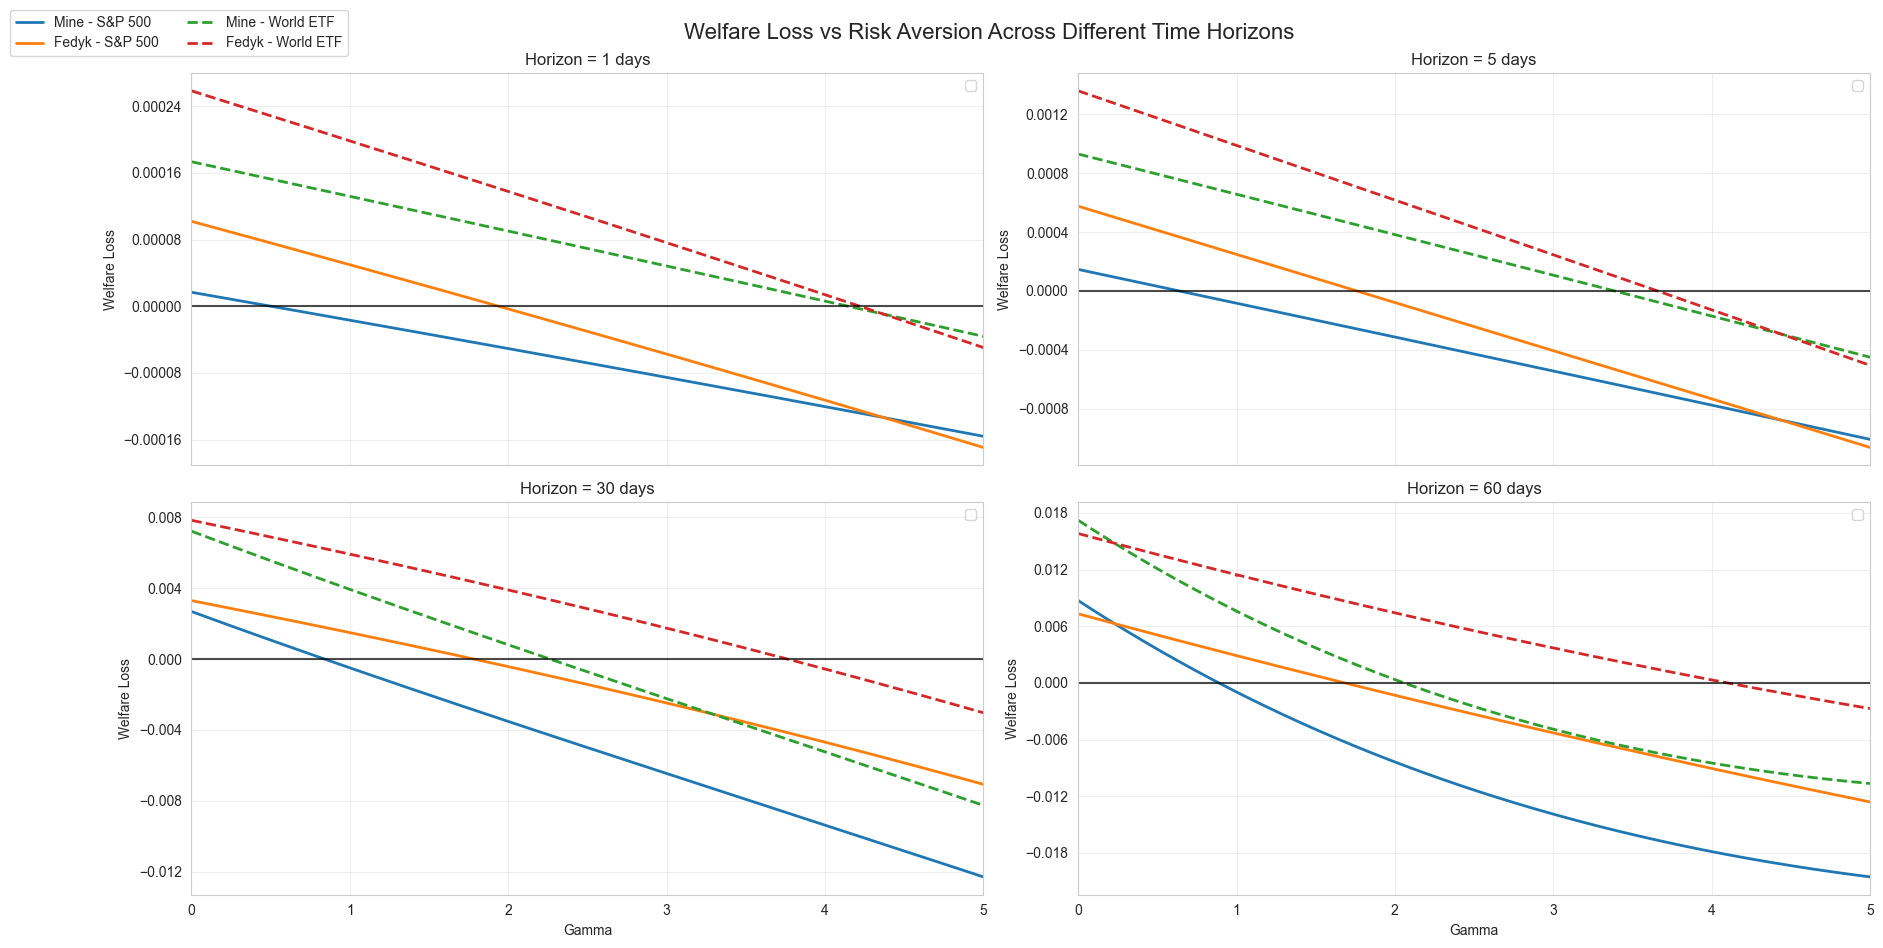
\includegraphics[width=\linewidth]{../images/wl_mkt.png}
\caption{Welfare loss of "Mine" and Fedyk Robinhood portfolios relative to the World ETF and S\&P 500 plotted as a function of the CRRA risk-aversion coefficient across 1-, 5-, 30-, and 60-day return horizons.}
\label{fig:wl_mkt}
\end{figure}    



\subsection{Implied Risk Aversion Approach}
\subsubsection{Deriving the Condition}
To address the limitations of our cutoff $\gamma$ approach, we turn to the canonical condition of maximizing expected utility by changing the share of wealth invested in the risky asset.  
In this framework, the agent decides to invest an amount $\alpha$ in the risky asset, his final wealth is therefore:
\begin{equation}
    W_1 = (1-\alpha) W_0 R_f  + \alpha W_0 \tilde R 
    \label{risky_portfolio}
\end{equation}
where $W_0$ is the initial wealth, which we can assume w.l.o.g equal to 1, $R_f$ is the gross return of the risk free asset and $\tilde R$ is the random variable that expresses the returns in the risky asset.

Defining $r=\tilde R - R_f$ we can approximate the CRRA utility of \ref{risky_portfolio} with a second-order taylor expansion around $R_f$:
\begin{equation}
    \mathbb{E}[U(W_1)] \approx R_f^{-\gamma} [\alpha \mathbb{E}[r] - \frac{\gamma}{2}\alpha^2\mathbb{E}[r^2]]
\end{equation} 

The investor chooses its portfolio to maximize the expected utility:
\begin{equation}
    \max_{0 \,\le\, \alpha \,\le\, 1}\; \mathbb{E}[U(W_1)]
    \;\approx\;
    \max_{0 \,\le\, \alpha \,\le\, 1}\;
    R_f^{-\gamma}\Bigl[\alpha\,\mathbb{E}[r]\;-\;\tfrac{\gamma}{2}\,\alpha^2\,\mathbb{E}[r^2]\Bigr]
\end{equation}

which yields the following equation\footnote{
    Derivation:
    $\text{FOC:}\quad
    \frac{\partial}{\partial \alpha}\Bigl\{R_f^{-\gamma}[\alpha\,\mathbb{E}[r]-\tfrac{\gamma}{2}\alpha^2\mathbb{E}[r^2]]\Bigr\}
    =
    R_f^{-\gamma}\bigl(\mathbb{E}[r]-\gamma\,\alpha\,\mathbb{E}[r^2]\bigr)
    \;=\;0$}:
\begin{equation}
    \alpha^*=
    \frac{\mathbb{E}[r]}{\gamma\,\mathbb{E}[r^2]}
\end{equation}

where $\mathbb{E}[r]=\mu-R_f$ and $\mathbb{E}[r^2]=\sigma^2+(\mu-R_f)^2$. 
Since returns are small, $(\mu-R_f)^2\ll\sigma^2$. We derive the following:
\begin{equation}
    \gamma^* = \frac{\mu-R_f}{\alpha \sigma^2}
    \label{gamma_star}
\end{equation}

In our case, both $\alpha$ and $\gamma$ are unknown. 
The variable of interest is $\gamma$, we can therefore use \ref{gamma_star} to compute it for every $\alpha$ in $[0,1]$. 


\subsubsection{Empirical Estimates and Interpretation}
\label{sec:gamma_estimates}
The results in this section might diverge slightly with the approach proposed above in section \ref{sec:cutoff} for a couple of reasons. 
First, here we limit investors preferences to the second moment, assuming directly that higher moments do not influence investor's utility.
Secondly the limited sample size, especially at longer horizons, limits the precision of the proposed estimates.
Moreover, in the \ref{sec:cutoff} section we implicitly assumed investors to hold all their wealth either in the Robinhood portfolio or in the market i.e.,
using this section's notation, to have $\alpha=1$.
Notwithstanding these challenges, some general conclusions can be drawn. 

A relevant point that should be discussed is the choice of not using rolling returns. 
Although they provide a good proxy for assessing the typical return over different horizons and across secruties, 
these return series suffer from autocorellation by construction, implying a very small variance especially at longer horizons.
Therefore, the risk aversion estimates provided by \ref{gamma_star} are unreliable and orders of magnitude greater than acceptable values in asset pricing.
For this reason, we focus or attention on daily, weekly, monthly and bi-monthly returns starting from the first day in the sample. This will avoid the problem with autocorrelation and provide interpretable and useful estimates over different horizons.

In table \ref{tab:gamma_implied} we report the implied share invested in the risky asset given a feasible upper and lower bound for investor's risk aversion, namely $\gamma=2$ and $\gamma=5$.
The full curves are plotted below in Figure \ref{fig:alpha_gamma}.
Something we should note is that since we have limited $\alpha$ to be in $[0,1]$ and $\sigma^2 \geq 0$, the implied risk aversion can be negative only if the mean excess returns are negative.
across all horizons.
As expected, $\alpha$ falls in a hyperbolic fashion, since \ref{gamma_star} implies $\alpha \propto \frac{1}{\gamma}$.

Across all four holding-period horizons and securities, lower risk aversion implies substantially higher optimal equity weights ($\alpha^*$) tha higher risk aversion.
Comparing across strategies, the S\&P 500 series has the largest implied shares at $\gamma=2$, rising from 0.766 at one day to 0.890 at five days before settling at 0.708 by sixty days, while its $\gamma=5$ allocations remain above both Robinhood strategies throughout. 
The World ETF's position at the bottom of the table highlights its lower excess-return profile: even at the longest horizon its $\gamma=2$ weight of 0.328 barely matches the $\gamma=5$ allocation to the Robinhood portfolios. 
Between the two Robinhood constructions, Fedyk is uniformly more aggressive than Mine, its $\gamma=2$ allocations exceed Mine's by roughly 10-25 percentage points at every horizon, reflecting Fedyk's higher expected excess return per unit variance.

\begin{figure}[H]
    \centering
    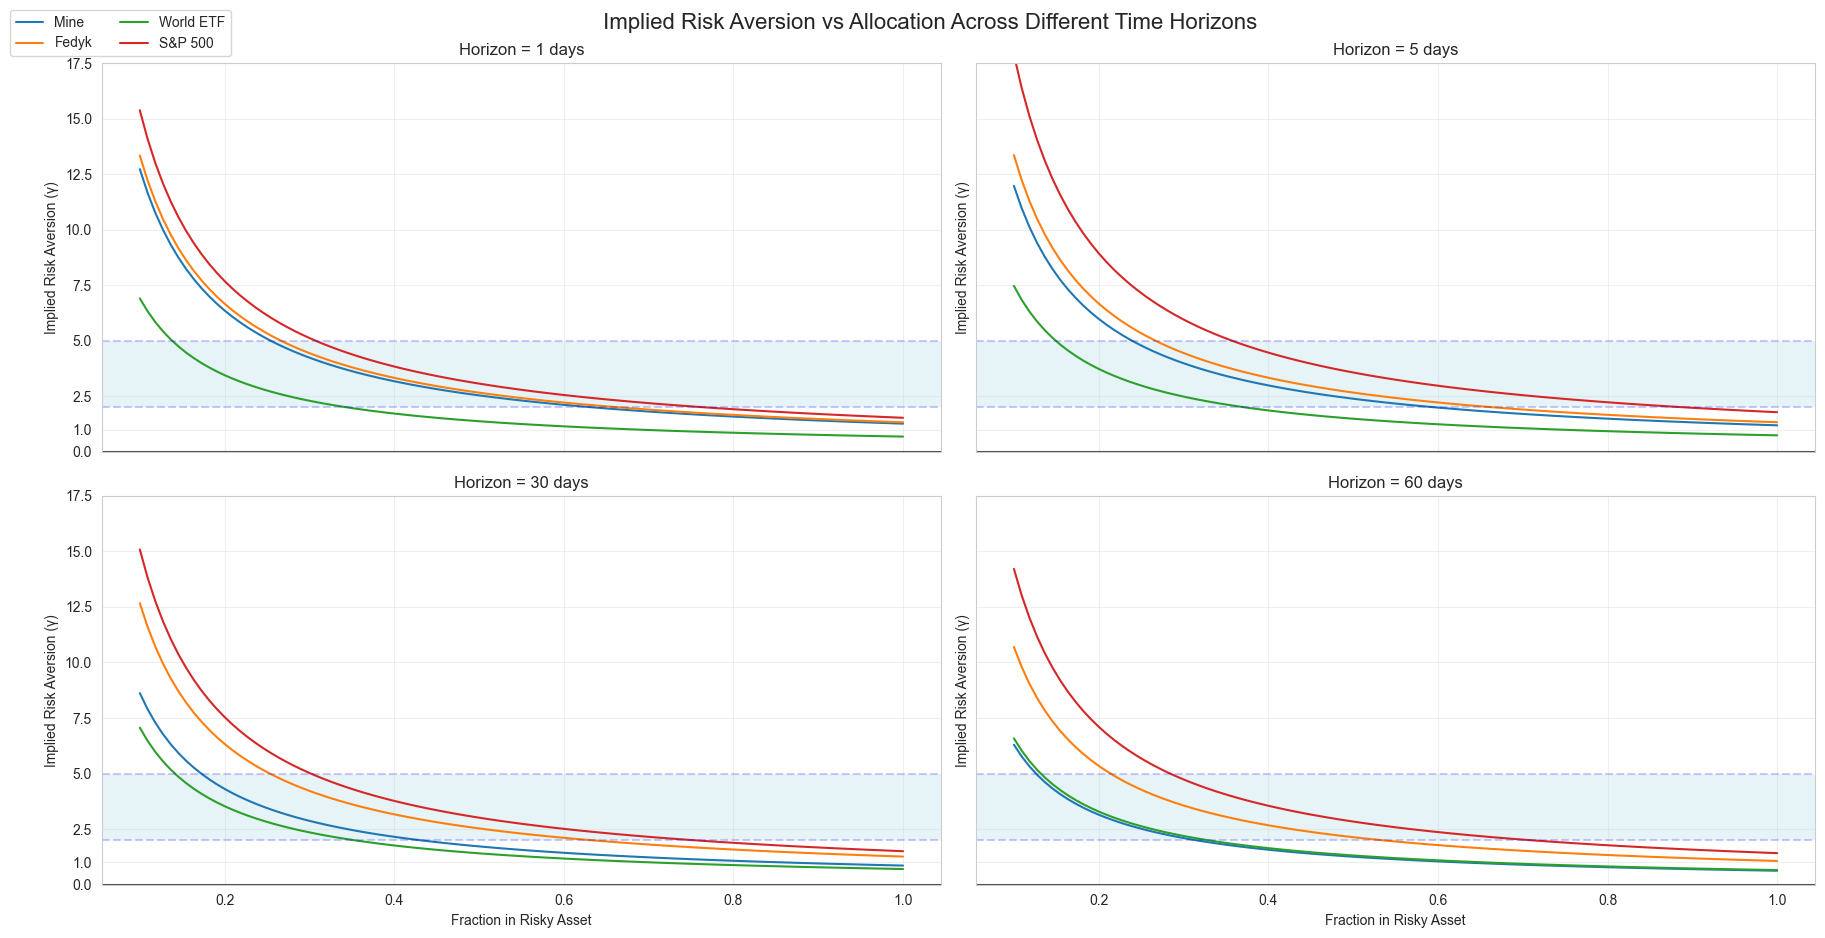
\includegraphics[width=\linewidth]{../images/alpha_gamma.png}
\caption{Implied CRRA risk aversion parameter as a function of allocation to each strategy (Mine, Fedyk, World ETF, S\&P 500) across 1-, 5-, 30-, and 60-day horizons. Shaded bands mark the typical empirical range of $\gamma \in [2,5]$.}
\label{fig:alpha_gamma}
\end{figure}    

This somewhat counterintuitive results can be interpreted by noticing that the condition we've set (\ref{gamma_star}) is simply a modified version of the Sharpe ratio.
It is rational for investors in this framework to allocate a greater portion of their wealth if the risky asset promises higher risk-adjusted returns.
The results are in table \ref{tab:sharpe_ratio}.